%%%%%%%%%%%%%%%%%%%%%%%%%%%%%%%%%%%%%%%%%
% ELEE	3720 Electromechanical Energy Conversion: Report template
% By Ratheesh Ravindran
%%%%%%%%%%%%%%%%%%%%%%%%%%%%%%%%%%%%%%%%%
\documentclass[12pt]{article}
\usepackage[english]{babel}
\usepackage[utf8]{inputenc}
\usepackage{amsmath}
\usepackage{graphicx}
\graphicspath{{Images/}}
\usepackage[colorinlistoftodos]{todonotes}
\usepackage{hyperref}

%\usepackage{fancyhdr}
%\pagestyle{fancy}
\begin{document}
\begin{titlepage}
\newcommand{\HRule}{\rule{\linewidth}{0.1mm}} 
\center % Center everything on the page
 
%---------------------------------------------------------------------------------
%	HEADING SECTIONS (Enter the Homework/assignment No., only)
%---------------------------------------------------------------------------------
\textsc{\Large MIDDLEWARE}\\[0.5cm] % heading course Number
\textsc{\Large Design et Autonomisation d'un kart }\\[0.5cm] % heading course name
\textsc{\large Projet }\\[0.5cm] % Minor heading
%---------------------------------------------------------------------------------
%	TITLE SECTION (Replace 'TITLE' with the Homework/assignment Name/title)
%---------------------------------------------------------------------------------

\HRule \\[0.4cm]
{ \huge \bfseries KART}\\[0.1cm] % Title of your Homework/assignment
\HRule \\[1.5cm]
 
%---------------------------------------------------------------------------------
%	AUTHOR SECTION (EDIT THE NAME and T.NO., only)
%---------------------------------------------------------------------------------

\begin{minipage}{0.4\textwidth}
\begin{flushleft} \large
Gwendal \textsc{Priser}\\  % Enter Your name and T.No.
\end{flushleft}

\begin{flushleft} \large
    Paul-Antoine \textsc{Le Tolguenec}\\  % Enter Your name and T.No.
    \end{flushleft}
    \begin{flushleft} \large
        Gwendal \textsc{Priser}\\  % Enter Your name and T.No.
        \end{flushleft}
\end{minipage}
\begin{minipage}{0.4\textwidth}
    \begin{flushleft} \large
        Gwendal \textsc{Priser}\\  % Enter Your name and T.No.
        \end{flushleft}

        \begin{flushleft} \large
            Gwendal \textsc{Priser}\\  % Enter Your name and T.No.
            \end{flushleft}
\end{minipage}\\[1cm]
{\large \today}\\[1cm] % Date, change the \today to a set date if you want to be precise

\includegraphics{ENSTA1246-524.png}% \\[0.5cm] % 
\vfill % Fill the rest of the page with white-space

\end{titlepage}
\include{GradingRubric}
\tableofcontents          % Required
\listoffigures
\listoftables
\newpage

% Do not edit the below sections, enter all details in respective chapters
% Add the images/screen-shorts to the image folder and insert them in the respective chapters


\section{Introduction}
\paragraph{}In the middleware module of UV 4.1, we are asked to implement the ROS middleware to drive a small car built in the previous semester. 
This small project consists in driving around an athletics track in an autonomous way. 
To carry out this project we have various sensors such as the Inertielle control unit which estimates the heading of the car and its acceleration, the camera, 
the gps which will allow us to estimate the position of the small car. We also have an on-board computer, in this case a raspberry.

\textbf{Repo GitHub}

\url{https://github.com/gwendalp/kart}



\section{Hardware}
\sesction{Hardware}

\subsection{Introduction}

\subsection{Main Board}
\paragraph{}For this project, we decided to use a \textit{Raspberry Pi 3B+}
as main board. It will let us plug some sensors and control the motors of
the car according to the wanted behavior we have programmed.

\paragraph{}On this Raspberry Pi, we need to choose an Operating System. our
choice was to use Ubuntu Mate because of its simplicity to install and its 
polyvalence. It will let us do everything we want, like plug sensors, code
any program to control our car, ... A preview of Ubuntu Mate is shown on
the ~\ref{fig:ubuntu}

\begin{figure}[!ht]
    \begin{center}
        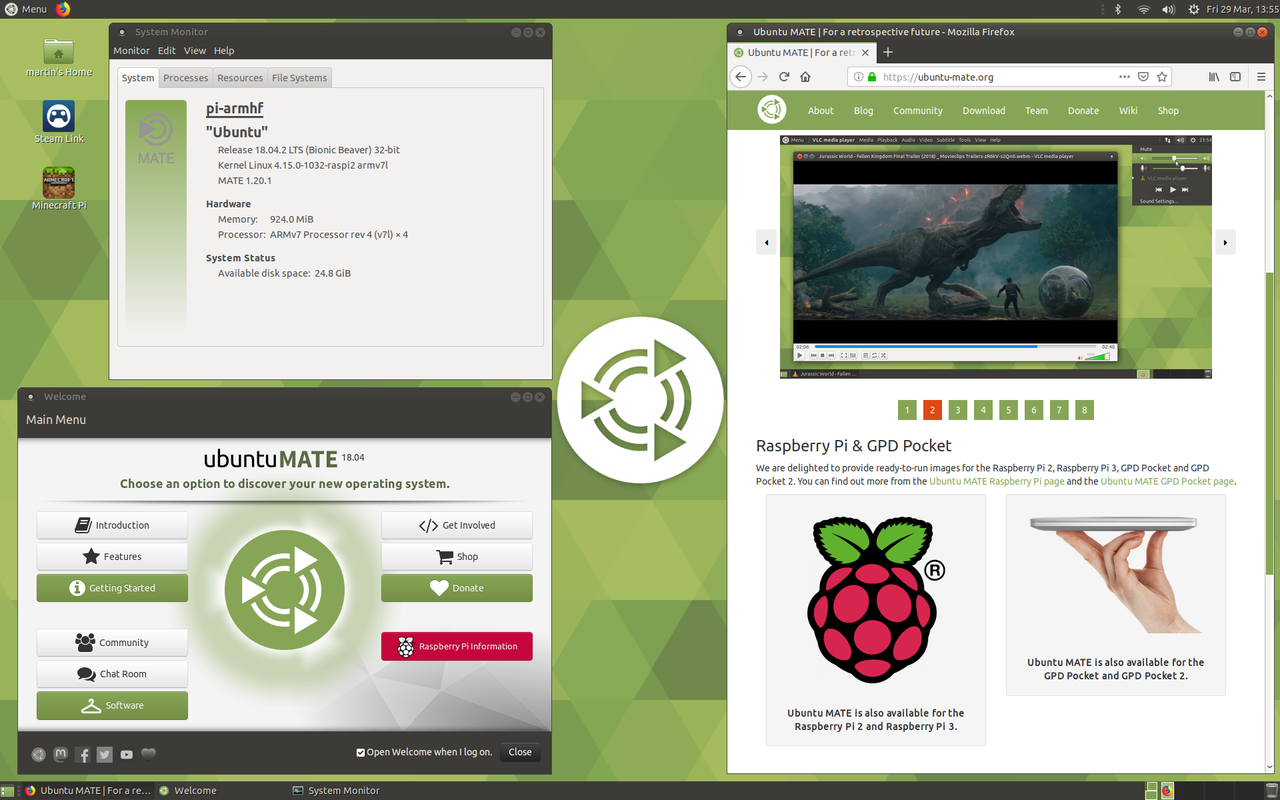
\includegraphics[scale=0.3]{Images/Ubuntu_mate.png}
    \end{center}
    \caption{Ubuntu Mate screen}
    \label{fig:ubuntu}
\end{figure}

\paragraph{}As an imposed figure for our project, we decided to use the 
\textit{Robot Operating System} (ROS) as Middleware for this car. It's
going to offer us some practical tools to code our pragrams easily.
There is also some usefull community shared tools like \textit{rqt}
or \textit{key\_telop} we will use in this project. Then we decided to
setup a graph node and to code these node in order to build our system
as shown on the following graph node.

\begin{figure}[!ht]
    \begin{center}
        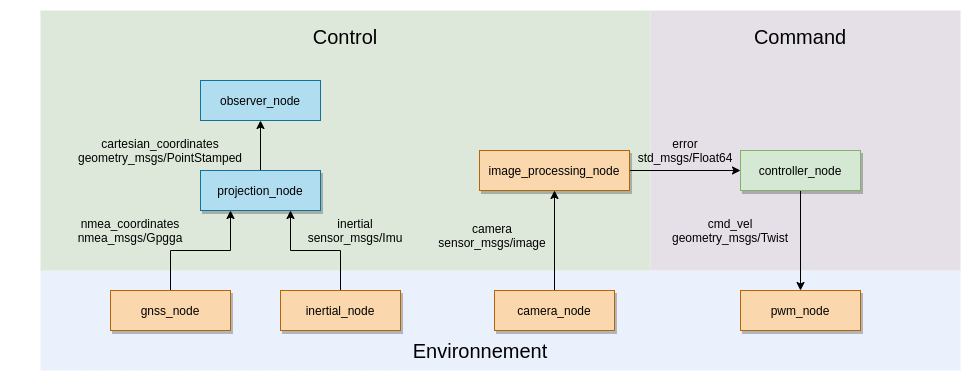
\includegraphics[scale=0.4]{Images/node_graph.png}
    \end{center}
    \caption{Graph node of the kart}
    \label{fig:graphnode}
\end{figure}

\subsection{Sensors}

\paragraph{}This section present the main hardware configuration of the car. 
For this project we have to choose which sensors we want in our 
car in the following list.

\begin{figure}[!ht]
    \begin{center}
        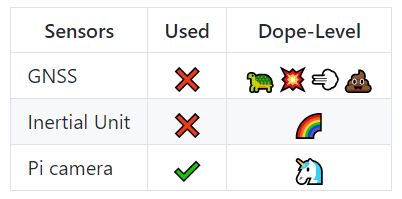
\includegraphics[scale=0.6]{Images/Sensors.png}
    \end{center}
    \caption{The Sensors list available on our GitHub}
    \label{fig:sensors}
\end{figure}

\paragraph{}
As it's shown we decided to choose neither the GNSS nor the Inertial 
Units, mainly because of their accuracy.

\paragraph{}
Actually, for our problem we found that an accuracy of 1 meter
for the \textit{GNSS} is too large because the car need to run in a 0.8 meter
wide racing lane, following a line. This sensors is alos not able to know if
the car position is correct.

\paragraph{}
For the \textit{Inertial Unit}, we found that this sensor is too noisy to
give us any usefull informations about the state of our car. For instance the
consecutive integration of the acceleration in order to get the speed and the
position of the car leads to an important drift effect on our data. So this
sensor is not currently able to to give any correct informations about the state
of the car. Moreover, the acceleration of the car could be quite good after filtering
if we only needed it. In our case the only usefull information is to know the
position of our car in relation to the line.

\paragraph{}
That's why we decided to focus our attention on the camera. Because
we are using a \textit{Raspberry Pi 3B+}, the camera we have choosen is the official 
camera which can be pluged on the dedicated port on the board. This sensor is
perfectly suited to our problem, because with an appropriated image processing
we will be able to detect the line and to correct the car trajectory.

\subsection{Configuration}
\paragraph{}
Now we will explain how we configured our sensors in our project, to
let them comunicate with the software and with the car.

\subsubsection{Pi Camera}
\paragraph{}
The configuration of the camera on the raspberry pi is relatively simple. We
used the \textit{raspi-config} utility to configure the camera. That's how we set up
the camera on the Raspberry Pi.

\begin{figure}[!ht]
    \begin{center}
        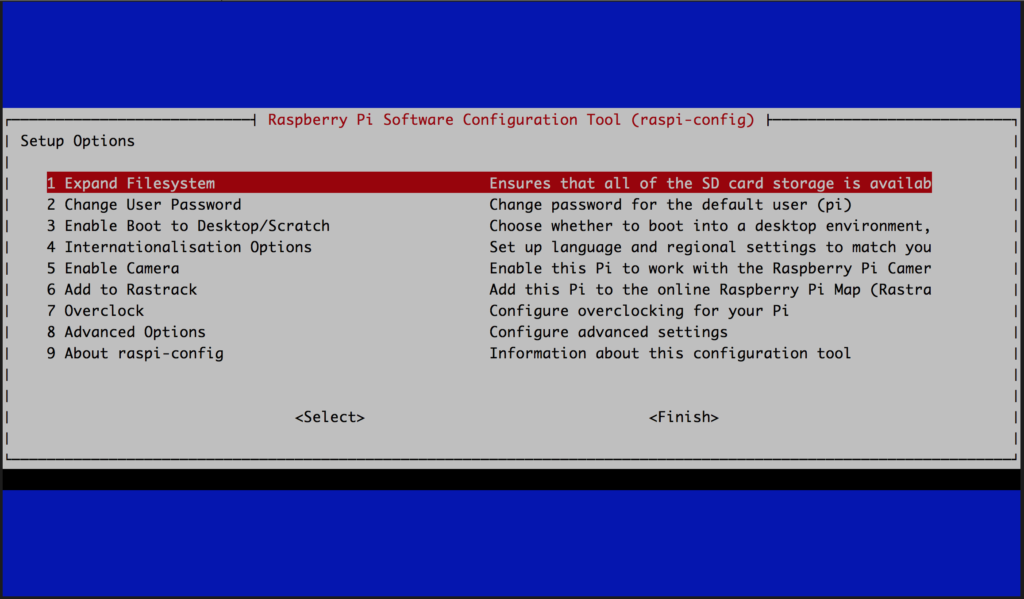
\includegraphics[scale=0.3]{Images/Raspi_config.png}
    \end{center}
    \caption{raspi-config utiliy on the Raspberry Pi}
    \label{fig:raspi_config}
\end{figure}

\subsubsection{Hardware PWM}
\paragraph{}
On Raspberry Pi board there is a lot of way to generate pwm signals.
The most of the time, these methods are software based and so they are not
accurate. With a lot of searches, we found a website who speak about the
raspberry pi's hardware pwm signals. There is apparently an hardware pwm
generator used by the bord to generate sounds. It's better to use hardware 
generated pwm, because if the processor has a slow down and the interrupt
is not correctly handled, the pwm duty cycle will not be very accurate and
the car will not be able for instance to follow a straight line, because the
bearing of the car is controled by a servomotor with a pwm signal.

\paragraph{}So we decided to use this tutorial : \cite{pi_pwm}, 
which explain us how to setup pwm signals on the Raspberry Pi,
and how to correctly configure the files to have a standard pwm signal
which is generated. Then we need to give the rights to users for reading and
writing in these files. All these bash command are in \textit{init\_pwm.sh}.

\paragraph{}
Then we have to add some automation. So we created a \textit{crontab} rule.
That will automatically create all the required files and allow the permissions
to every users. We just have to write in the file \textit{duty\_cycle} a value between
$1.000.000$ and $2.000.000$, and the Raspberry Pi will read and adjust pwm signals
in real time.

\paragraph{}
Last but not least, we setup an autologin in order to open a session automatically
when the Raspberry Pi boot. That's very usefull in order to launch our programms
easily on boot and without any keyboard, mouse or monitor.

\section{Image Processing}



\paragraph{}
To carry out the image processing we used very simple theoretical notions. The library we used is open cv. The figure below summarizes our image processing.
\begin{figure}[ht!]
    \begin{center}
        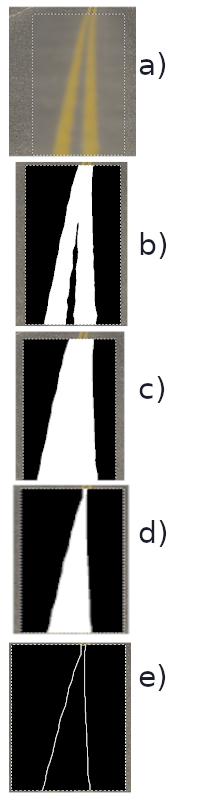
\includegraphics[scale=0.3]{Images/diagramme.png}
    \end{center}
    \caption{image processed}
    \label{fig:img_processing}
\end{figure}

\subsection{Data logging}
\paragraph{}
For the first part of this image processing, we had to collect images.
So first we went into the environment in which the robot was going to evolve.

\begin{figure}[ht!]
    \begin{center}
        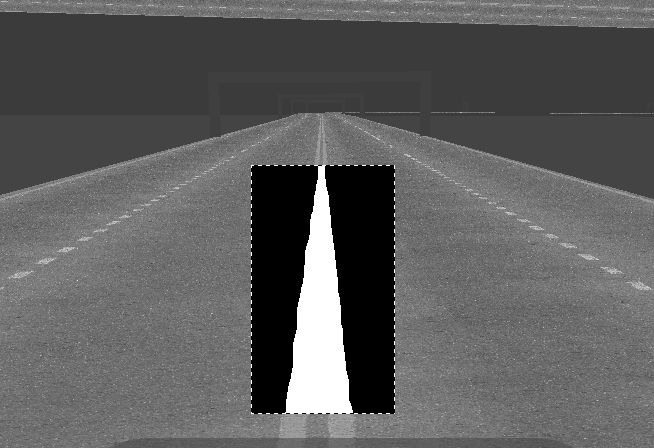
\includegraphics[scale=0.3]{Images/image_process.png}
    \end{center}
    \caption{image processed}
    \label{fig:img_processing}
\end{figure}

\subsection{pre binarization treatment}
\paragraph{}
In this part, we first had to perform a pre-binarization treatment in order to reduce post-binarization noise.
So we used a Gaussian filter to blur the image.

\subsection{binarization}
\paragraph{}
Since the line we wanted to mark is white. An effective treatment is simply to switch to grey level. 
So for binarization, we switch the image to a grey level and threshold for a grey level that we have determined empirically.

\subsection{post binarization treatment}
\paragraph{}
In this part we performed a morphological treatment. There was still a lot of noise after binarization. So we made an opening. 
With a kernel in the shape of a rectangle (since it was the most efficient for this treatment).
At the end of this treatment we obtain a well defined line which crosses the screen.

\subsection{find the center of the line}
\paragraph{}
In this last part, the contours are marked using a gradient method. Then the contours are sorted from the smallest to the largest.
We recover the largest contour.
And we recover the coordinates of the barycentre of the contour.
Then the error is the difference between the center of the image and the coordinates of the pixel.
The problem with this method is that with the barycentre we have a regulation on a point in the centre of the image. And therefore, we don't use all the data we have.
So we decided to use the highest points of the contour.
Indeed, the position of the center of the line at the highest point of the image gives us an idea of the evolution of the road at the moment. From now on we use the horizon. It allows us to get information further into the "future". And so it allows for better regulation and therefore to go faster.


\section{Explications}



\section{Resultats}
\input{Chapters/04_Results}

\section{Discussions et Conclusion}
To conclude, we think that we already have a strong basis for this project, particularly
with the ROS structure  which is already setup. Then we have to perform test with the
real system because the simulation is correctly working and a good proof of concept, 
but we lnow too that simulation and reality are always different. We have to do some
improvements on our projetc too, like adding an mission controler in order to control the
robot in some cases where we couldn't use the line following command, for instance when the 
camera is not seeing any lines, and we ha to add a GUI in order to show the kart state
like his position, is speed and the circuit.

%\bibliographystyle{plain}
%\bibliography{Bibliography.bib}

\appendix
\section{Appendix}
\input{Chapters/06_Appendix1}


%---------------------------------------------------------------------------------
%	Example SECTION (Remove this section to finalize the report.

% Remove this line to finalize the report.
%---------------------------------------------------------------------------------


\end{document}


% Note: Again, you don’t need to answer just the above questions. They are being provided to give you a flavor of what is required for each section. Use your judgment and initiative to add or subtract based on the specific homework. You can add any other conclusion or discuss any other aspect of your effort that you think it is important to highlight.

% Also ensure to attach the MATLAB or MULTISIM files with this report